% Section content template for individual Educative lessons
% This file contains the actual content for a specific section
% Generated from Educative API section content

% Section: System Design Primer
% Section ID: 6123745074610176
% Section Slug: system-design-primer
% Generated: 2025-12-08T15:41:51.181608

In the previous chapter, we introduced the fundamentals of System Design and its core characteristics. In this lesson, we will build on the foundation by exploring the fundamental principles of operating systems, networking, and advanced concepts in distributed systems. These are the topics that frequently appear in System Design discussions and interviews.

\begin{figure}[htbp]
 \centering
 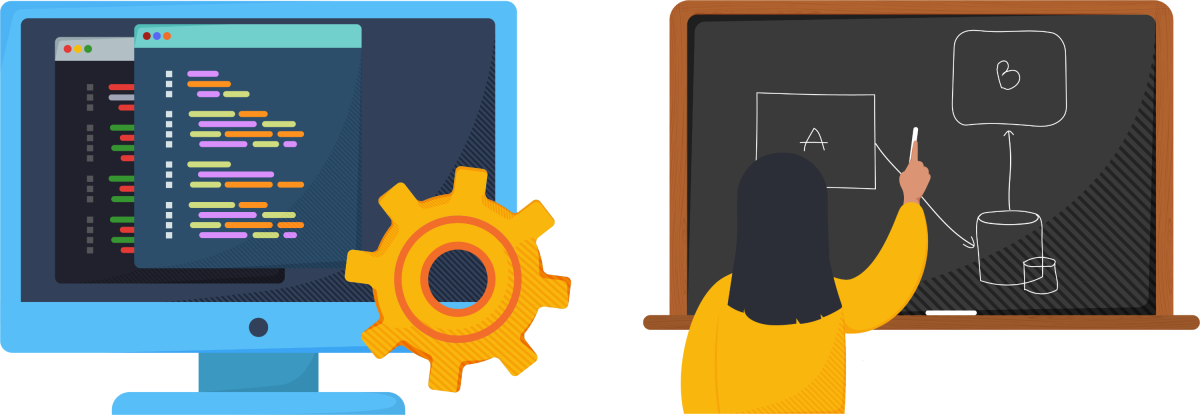
\includegraphics[width=0.25\textwidth]{Images/chapter_44/section_6123745074610176/4877747362856960.png}
 \caption{Other interviews vs. a System Design interview}
\end{figure}

The origins of System Design can be traced back to the early days of computing, with pioneers like Edsger W. Dijkstra laying the groundwork for structured programming and modular design principles.

\textbf{Disclaimer:} This chapter provides an overview of the basic distributed system concepts. If you are already familiar with these topics, you can proceed to the next chapter. However, we recommend quickly reviewing this chapter to refresh your knowledge.
\\
Of course, there are several terms and concepts in System Design. However, based on our experience, the following topics are considered the highest priority for building a strong understanding.

\subsection{Operating systems fundamentals}\label{DiZZWmflUnRCpegfXzJiy}
\\
\textbf{Operating systems (OS)} are the backbone of modern computing, but their role extends far beyond simply running applications.
\\
For system designers, a deep understanding of OS internals is crucial. This includes knowledge of process management, memory allocation, concurrency models, and file systems. Familiarity with different OS architectures (e.g., monolithic, microkernel) and their performance implications can also be invaluable in making informed design decisions.
\\
A deep understanding of operating system (OS) concepts is non-negotiable in System Design.
\\
From scheduling and resource allocation to process management and concurrency models, these foundational principles empower us to craft robust, efficient, and scalable systems. Let 's dive into the essential OS knowledge needed to elevate our System Design skills.

\subsubsection{Concurrency}\label{JxdZ1z8OidoctYsJ0gveh}
\\
\textbf{Concurrency}, the simultaneous execution of multiple tasks, is a fundamental challenge and opportunity in System Design. While processes(A single instance of a program) and threads(Processes run on threads, often called the smallest unit of execution) are the building blocks, the true mastery lies in understanding how to orchestrate them effectively to achieve optimal performance, reliability, and responsiveness.
\begin{quote}
\textbf{Educative byte:} \emph{Concurrency is a way to structure a software system by decomposing it into components that can be executed independently---\textbf{Rob Pike, co-creator of the Go programming language}}
\end{quote}
\\
Modern computing environments, particularly distributed systems such as web farms and cloud infrastructure, heavily rely on concurrency to achieve scalability and optimal performance. However, this concurrency necessitates robust thread synchronization and coordination mechanisms to ensure data consistency, prevent race conditions(A race condition occurs when two or more threads can access shared data and they try to change it at the same time.), and manage resource contention.

\begin{itemize}
\item
\protect\phantomsection\label{z6iUI0mCRRrtkmT-ucgUM}
\textbf{Locks:} This is the most fundamental synchronization primitive. Various types of locks exist, including mutexes (mutual exclusion locks), read-write locks, and spin locks, each with distinct performance characteristics and use cases.
\item
\protect\phantomsection\label{SssVwsokEk_D9FQaZkjol}
\textbf{Semaphores:} These are generalized locks that allow a limited number of threads to access a resource concurrently. Semaphores are often used to control access to a pool of resources or to implement producer-consumer scenarios.
\item
\protect\phantomsection\label{k1Wbq75uSvLBDjVHGUz1G}
\textbf{Condition variables:} These enable threads to wait for a specific condition to become true before proceeding. Condition variables are typically used with locks to create more complex synchronization patterns.
\item
\protect\phantomsection\label{JUYTg2uxQ5hIyNQsbmcOH}
\textbf{Barriers:} These are synchronization points where threads wait until all threads in a group have reached the barrier before continuing. Barriers are useful for coordinating the execution of parallel tasks that must be completed in phases.
\end{itemize}

Multithreading (running multiple processes in parallel) first appeared in the 1950s, and simultaneous multithreading (SMT) was investigated by IBM in 1968.

However, there is one common issue with concurrency: synchronization.

\subsubsection{Synchronization}\label{clqQMNtp3U5qFJLvqrozp}
\\
When two independent processes run in parallel, synchronization is not a problem (they do not share resources).
\\
However, when dealing with dependent processes, synchronizing them is crucial to achieving successful concurrency. \textbf{Synchronization} is the cornerstone of concurrent programming. It's the art and science of coordinating access to shared resources among multiple processes.
\\
Just as traffic lights manage the flow of vehicles, synchronization mechanisms like mutexes (mutual exclusion locks), semaphores, condition variables, and monitors, each with unique strengths and use cases, regulate access to shared data. Choosing the right mechanism ensures correctness and performance in concurrent systems.

\begin{figure}[htbp]
 \centering
 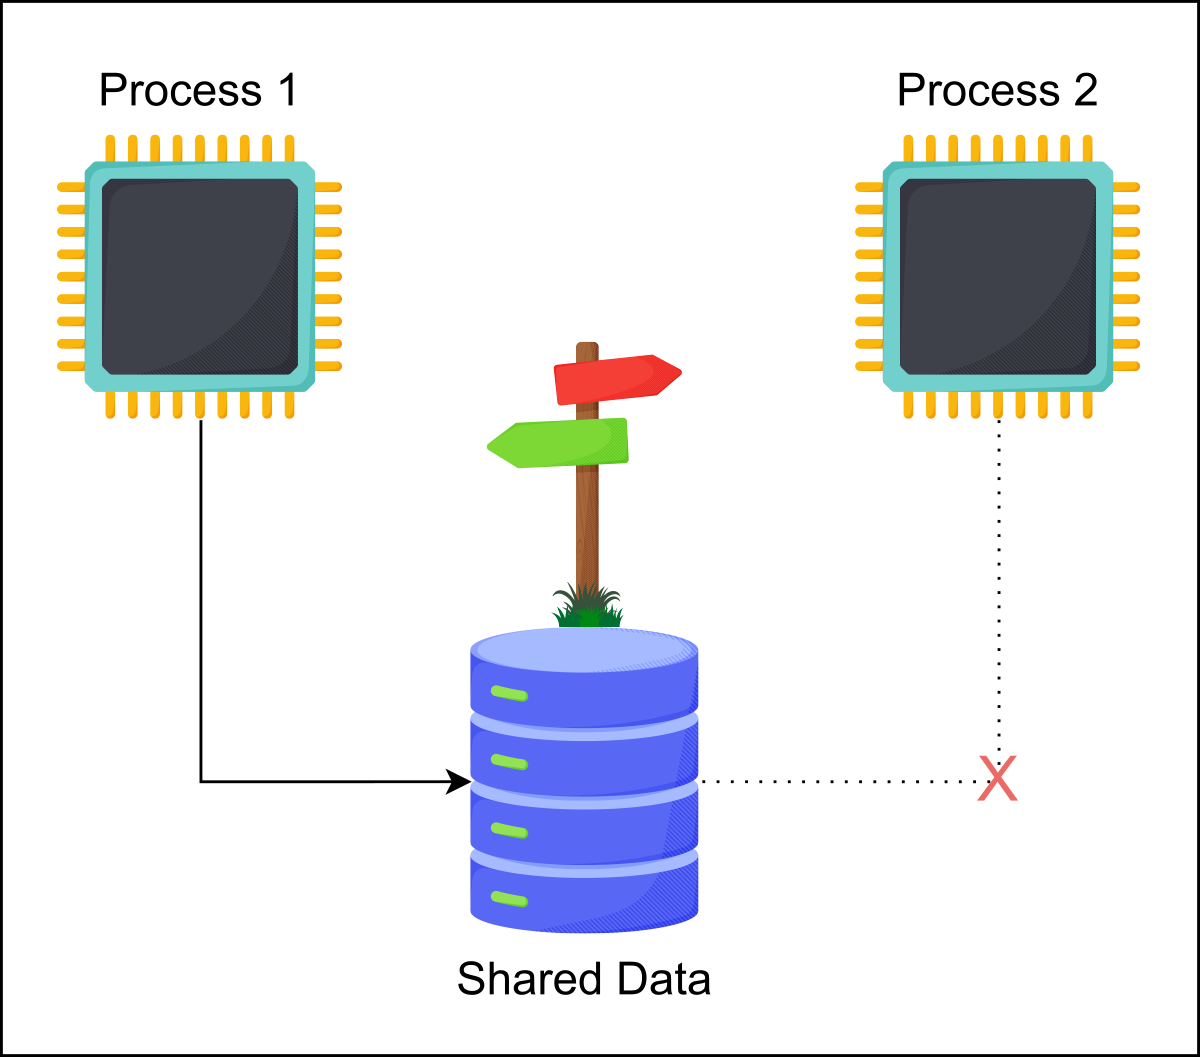
\includegraphics[width=0.15\textwidth]{Images/chapter_44/section_6123745074610176/6559109534842880.png}
 \caption{Process 1 needs the shared data, so it has acquired a lock on it. This means Process 2 cannot access the data until Process 1 is done using it.}
\end{figure}

We use interprocess communication (IPC)(Interprocess communication is a mechanism provided by the operating system that allows processes to communicate and synchronize their actions through methods like shared memory and message passing.)to synchronize and communicate messages between different processes. This is where the \emph{traffic lights} come in. One process can broadcast a message to the others about using/locking a resource, or about no longer using that resource.
\begin{quote}
\textbf{Note:} Understanding synchronization is critical. In a System Design interview, being able to discuss why a certain synchronization mechanism was chosen and what trade-offs it implies demonstrates a deeper level of understanding.
\end{quote}
\\
Distributed systems introduce additional challenges due to the lack of shared memory and the potential for network delays and failures. Several algorithms have been developed to address these challenges:

\begin{itemize}
\item
\protect\phantomsection\label{fbGVNxFEPPo-PAgouIfRv}
\textbf{Distributed locks:} These implement mutual exclusion in a distributed environment. Common approaches include centralized coordinator-based locks, token-based locks, and quorum-based locks.
\item
\protect\phantomsection\label{DsehXau9YGQKTXlD9a0pd}
\textbf{Lamport's logical clocks:} These provide a way to order events in a distributed system without relying on physical clocks. Logical clocks are used to ensure causal ordering and to detect inconsistencies.
\item
\protect\phantomsection\label{jMRPy2vW6w0e6gefT0-3n}
\textbf{Vector clocks:} These are an extension of Lamport's logical clocks that provide a more accurate representation of causality in distributed systems. Vector clocks are used in applications like conflict resolution in distributed databases and collaborative editing tools.
\item
\protect\phantomsection\label{Xp7eVGrOuwGPHt853VGG6}
\textbf{Paxos and Raft:} These are consensus algorithms that enable a group of distributed processes to agree on a single value even in the presence of failures. Paxos and Raft are utilized in distributed databases, file systems, and other systems that require strong consistency guarantees.
\end{itemize}
\\
While modern operating systems excel at managing concurrent processes on a single machine, their capabilities are inherently confined to that one system. This limitation can be overcome by harnessing the power of computer networks, which enables the distribution of processes across multiple machines and unlocks new levels of parallelism and scalability.

\subsection{Computer network essentials}\label{pbuIydLLO-CRheNO7ib8-}
\\
A computer network is a collection of interconnected devices that can share information and resources. It is a way for two independent systems to communicate. They are like IPC but for separate machines. The machines that need to communicate are usually connected through a LAN(Local Area Network), and messages are sent through the LAN infrastructure.
\\
How nodes(These are the individual devices connected to the network, such as computers, servers, routers, and switches.) are interconnected defines the network's topology, which can significantly impact performance, reliability, and cost. Common topologies include:

\begin{itemize}
\item
\protect\phantomsection\label{bd5nXhfgqwqKfNTcjoaVb}
\textbf{Bus topology:} A single cable (the bus) connects all nodes linearly. It is simple and inexpensive but vulnerable to single points of failure.
\item
\protect\phantomsection\label{R8hBZc1h5WTZGZjh-h22h}
\textbf{Star topology:} Each node connects to a central hub or switch. Offers better fault tolerance than bus topology but requires more cabling.
\item
\protect\phantomsection\label{OIfucZUB2BwRl1c9iYEHa}
\textbf{Ring topology:} Nodes are connected in a circular chain, with data flowing in one direction. Offers good fault tolerance and predictable performance, but can be complex to manage and maintain.
\item
\protect\phantomsection\label{1hcY2fFPy31wHqi4TYzwJ}
\textbf{Mesh topology:} Nodes are interconnected with multiple redundant links. Highly reliable and fault-tolerant, but expensive to implement.
\end{itemize}

\begin{figure}[htbp]
 \centering
 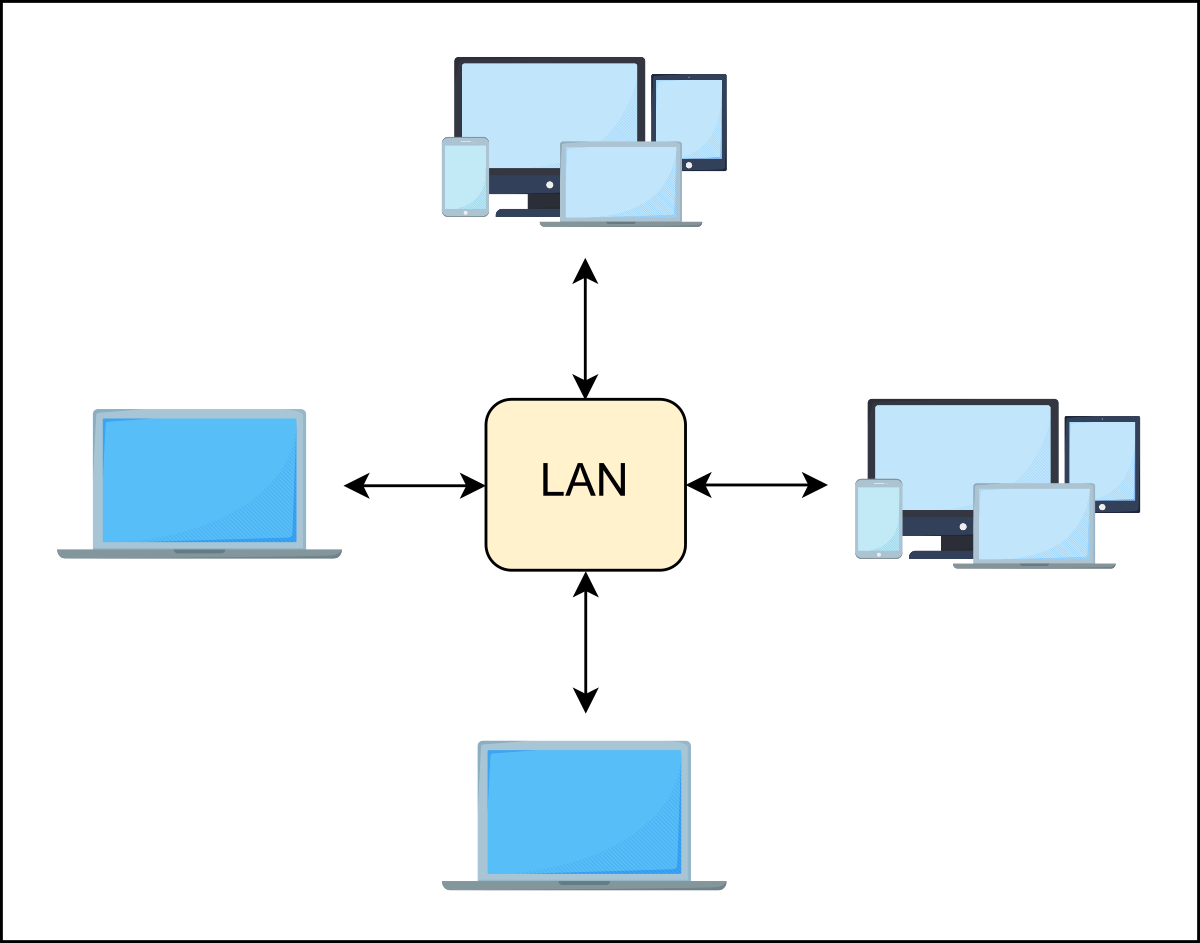
\includegraphics[width=0.15\textwidth]{Images/chapter_44/section_6123745074610176/6140817032740864.png}
 \caption{A group of machines interconnected through a LAN.}
\end{figure}

When sending messages through the network, we must be very specific in crafting those messages. These messages must pass through several hurdles (routers, switches, etc.), and a message meant for machine X mustn't arrive at machine Y.
\\
We can see why this would confuse the machines if it were to happen.
\begin{quote}
\textbf{Note:} Computer networks form the backbone of the internet, the infrastructure for System Design. Knowing the concepts of computer networks allows us to delve deeper into the implementation details.
\end{quote}
\\
The OSI(Open Systems Interconnection) model divides network tasks (Network tasks are the various operations and processes involved in that facilitate communication and data exchange between devices across a network. These tasks include data encapsulation, addressing, routing, error detection, and flow control.)into seven layers. Each layer has a specific job, from the physical wires (Layer 1) to our application (Layer 7). It 's like a layer cake, with each layer depending on the one below it. This completes the model of inter-machine communication for both LANs and cross-network (sometimes referred to as WAN(Wide Area Network)) applications.
\\
Let's look at an example of how all of this works.

\begin{figure}[htbp]
 \centering
 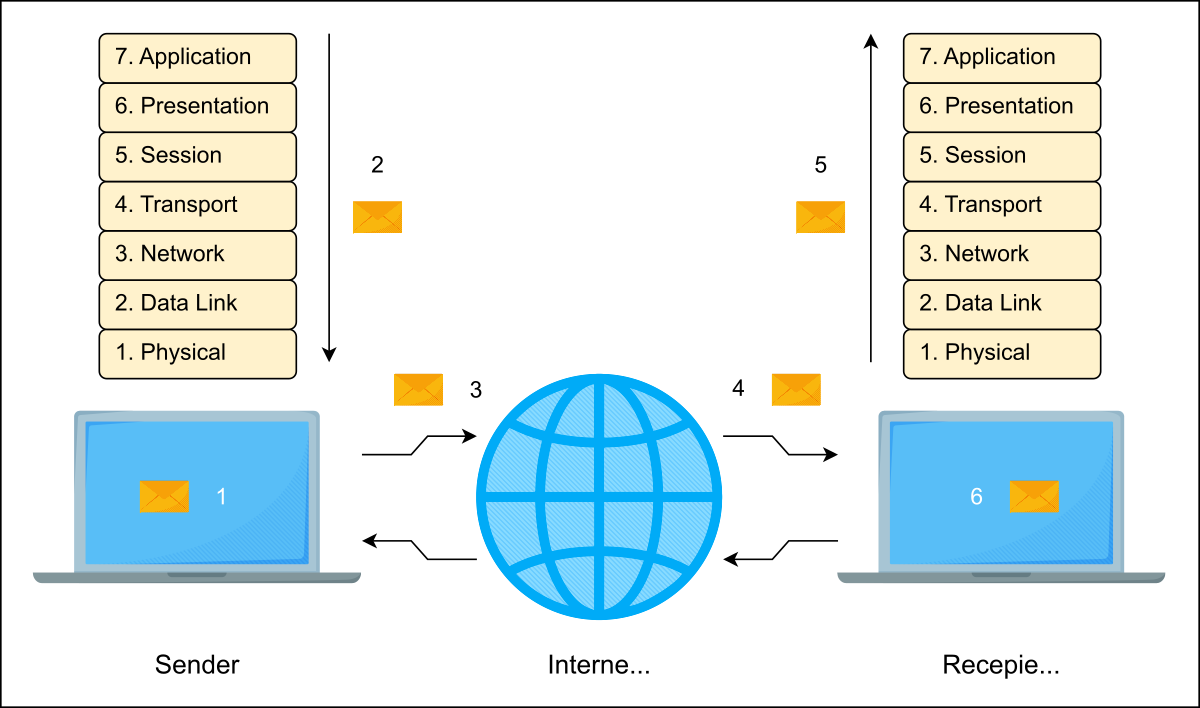
\includegraphics[width=0.5\textwidth]{Images/chapter_44/section_6123745074610176/5218477587431424.png}
 \caption{Sending a message over the internet.}
\end{figure}

To achieve this, the two key protocols for network-based communication are TCP(Transmission Control Protocol, is a core communication protocol for the internet that ensures the reliable and ordered delivery of data between devices. It works with the Internet Protocol (IP) to establish a connection, break data into packets, and ensure they are reassembled correctly at the destination.) and UDP(User Datagram Protocol, is a fast, connectionless communication protocol for sending data over the internet. It is used for time-sensitive applications like video streaming, gaming, and DNS lookups because it prioritizes speed over reliability, meaning it doesn\textquotesingle t guarantee data delivery, order, or error checking.).

\subsubsection{Transport layer protocols}\label{SgvO6w_Z5mUbiSbnpSua_}
\\
If computer networks are like the highways of the digital world, then network communication protocols are the traffic rules of the digital world.
\\
They govern how data travels, ensuring it reaches its destination efficiently and accurately. Think of TCP as the postal service; it ensures our data arrives reliably, in the right order, and with a confirmation. UDP is more like an announcer, quickly sharing information without verifying that everyone has heard it.
\\
TCP is used for tasks such as email and web browsing, where accuracy is crucial.
\\
UDP is used for live video streaming, where speed is more important than perfect delivery. Now , what if we want two devices on separate networks to communicate with each other? Let's look at application layer protocols.

\subsubsection{Application layer protocols}\label{7ZFltrSdpldZaAzwZux2f}
\\
HTTP(Hypertext Transfer Protocol) is the language our browsers use to communicate with websites. It allows us to request web pages and send data back.
\\
In this scenario, our machine, which is the browser, requests information from another machine located elsewhere. It 's a bit like a conversation, with each request and response forming a step in the dialogue. Whenever we have cross-network communication, we can be certain that HTTP is involved.

\begin{figure}[htbp]
 \centering
 
\includegraphics[width=0.15\textwidth]{Images/chapter_44/section_6123745074610176/4832023950262272.png}
 
\end{figure}

This protocol started the revolution for apps on the internet. Everything from social media and emails to online games uses HTTP.
\\
HTTPS(Hypertext Transfer Protocol Secure) builds on this foundation by providing a secure, encrypted connection, ensuring data privacy and integrity for all internet communications. FTP(File Transfer Protocol) and SMTP(Simple Mail Transfer Protocol), two other fundamental protocols, also play crucial roles in shaping the internet as we know it today. FTP enables the transfer of files between servers and clients, facilitating the sharing and distribution of digital content.
\\
SMTP, on the other hand, is responsible for delivering emails, enabling users to communicate with each other worldwide.
\begin{quote}
\textbf{Note:} When designing APIs in a System Design interview, one of the most frequently asked questions is which version of HTTP to use (HTTP/1.1 or HTTP/2.0) and why.
\end{quote}
\\
With the advent of the internet, communication between different machines became essential. Everyone started to find better and safer ways to communicate between networks. That 's how we got RPCs(Remote Procedure Calls) and APIs.

\subsubsection{Web API architectures}\label{3TPgO27HdkRDNPZCY8c62}
\\
We have likely heard of terms like REST(Representational State Transfer) and GraphQL as the essentials for any web application.
\\
\textbf{REST} is an architectural style for designing networked applications. It relies on a stateless, client-server communication model and leverages HTTP protocols, making it a highly scalable and flexible approach for building APIs.
\\
This simplicity and wide adoption have made REST a cornerstone of modern web development, facilitating seamless integration between diverse systems.
\\
GraphQL, on the other hand, is a query language for APIs and a runtime for executing those queries by using a type system we define for our data. It offers a more efficient, powerful, and flexible alternative to REST. With GraphQL, clients can request the data they need, reducing over-fetching and under-fetching of data.

REST and GraphQL are not mutually exclusive; they can be used together in a single application, leveraging the strengths of each where appropriate.

These frameworks are so essential for web development that we now have entire system architectures built to support them. While REST is powerful, RPCs can be superior in some applications.

\subsubsection{Remote procedure call frameworks}\label{iAPF6LF5q91eaPZwzbRYN}
\\
RPCs allow a program on one computer to execute a function or procedure on another computer as if it were running locally. The request message is sent to the remote computer, which executes the requested function and sends back a response message.

\begin{figure}[htbp]
 \centering
 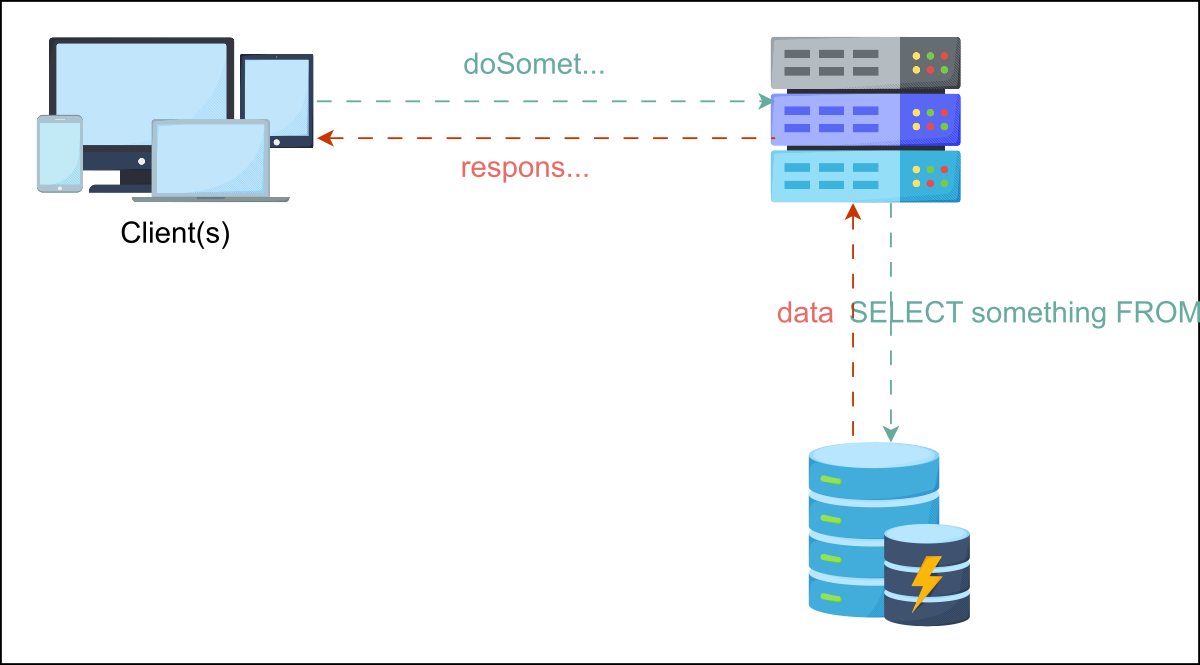
\includegraphics[width=0.5\textwidth]{Images/chapter_44/section_6123745074610176/6259281709891584.png}
 \caption{How RPCs work}
\end{figure}

RPCs are used in various applications, from distributed file systems to web services. They simplify the development of distributed systems by abstracting away the details of network communication.
\\
gRPC(Google remote procedure calls) is a high-performance, open-source RPC framework developed by Google. It leverages modern technologies like Protocol Buffers(This is a language-neutral way to serialize structured data.) and HTTP/2(This is a faster, more efficient version of the HTTP protocol.).
\\
gRPC offers several advantages over traditional RPC:

\begin{itemize}
\item
\protect\phantomsection\label{eEkkYRVyfr6GMAlWih9Vc}
\textbf{Performance:} gRPC is designed for high throughput and low latency, making it ideal for modern microservices architectures.
\item
\protect\phantomsection\label{dxXnUbfKmevkPNtttItep}
\textbf{Language:} gRPC supports various programming languages, allowing us to build distributed systems using our preferred tools.
\item
\protect\phantomsection\label{ygOE0mWcPbrKOYBS1vQTW}
\textbf{Streaming:} gRPC supports client-side and server-side streaming, enabling efficient communication for real-time applications.
\end{itemize}
\begin{quote}
\textbf{Note:} While gRPC offers numerous advantages,~it's important to consider its learning curve and additional tooling requirements before adopting it.
\end{quote}
\subsubsection{Comparison of the network protocols}\label{fdVw4sVTpNOzPFpQUNFcR}
\\
There are numerous network communication protocols, each designed for a specific purpose. The most popular ones are listed below.

\begin{center}
\begin{tabular}{|l|p{3.5cm}|p{3.5cm}|p{3.5cm}|p{3.5cm}|}
\hline
\textbf{Protocol} & \textbf{Description} & \textbf{Use Cases} & \textbf{Strengths} & \textbf{Weaknesses} \\
\hline
\textbf{TCP} & Provides reliable, ordered delivery of data. & Web browsing, email, and file transfer & It is reliable and guarantees data delivery. & It is slower than UDP due to error checking and retransmission overhead. \\
\hline
\textbf{UDP} & Provides fast, connectionless delivery of data. & Video streaming, online gaming, and DNS lookups & It is fast, with low latency. & It is unreliable and may drop packets, unsuitable for applications requiring guaranteed data delivery. \\
\hline
\textbf{HTTP} & Used for transferring hypertext (web pages). & Web browsing and APIs & It is simple and widely supported. & It is stateless, and each request/response is independent; it can be inefficient for frequent communication. \\
\hline
\textbf{REST} & Allows stateless communication between devices. & Public APIs, microservices, and web applications & It offers simplicity, ease of use, wide adoption, and scalability. & It presents an over-fetching/under-fetching issue. \\
\hline
\textbf{GraphQL} & Query language for APIs. & Complex client-server applications (mobile and web) & It offers precise data fetching, flexibility in evolving APIs, and strong typing. & It offers a steep learning curve, harder to implement caching. \\
\hline
\textbf{RPC} & Enables a program on one computer to execute a procedure on another computer. & Distributed systems, microservices, and remote file systems & It simplifies the development of distributed systems and abstracts network communication details. & If not implemented properly, it can be slower than local procedure calls and potential security vulnerabilities. \\
\hline
\textbf{gRPC} & A high-performance, open-source RPC framework. & Microservices, cloud-native applications, and real-time communication & It is efficient, language-neutral, and supports streaming. & It presents a steeper learning curve than simpler protocols requiring additional tooling. \\
\hline
\textbf{WebSocket} & Enables full-duplex communication over a single TCP connection. & Real-time web applications, chat applications, and collaborative editing & It offers real-time communication and efficient use of network resources. & It is more complex to implement than HTTP and may not be supported by all clients/servers. \\
\hline
\end{tabular}
\end{center}


Now that we have reviewed the various protocols that govern how data is sent, we can examine the high-level architectural patterns that define who communicates. These protocols serve as the foundation for more comprehensive communication models.

\subsubsection{Communication models}\label{5ubhEdmF9HqQn_tf2klCp}
\\
In the \textbf{client-server} model, communication is structured with distinct roles for clients and servers.
\\
Clients request services or resources, while servers provide these services or resources to them. This centralized approach is prevalent in various applications, including web services, email, and database management systems.
\\
The client-server model simplifies management and scaling, but it can also create a single point of failure if the server goes down.

Peer-to-peer systems can be traced back to 1969, while client-server systems appeared in the 1980s.

Conversely, the P2P(Peer-to-peer) model distributes the roles more evenly.
\\
Each peer can act as both a client and a server, sharing resources directly with others. This decentralization enhances redundancy and resilience, making P2P networks ideal for file sharing, blockchain, and collaborative applications.
\\
However, P2P can be more complex to manage.

\begin{figure}[htbp]
 \centering
 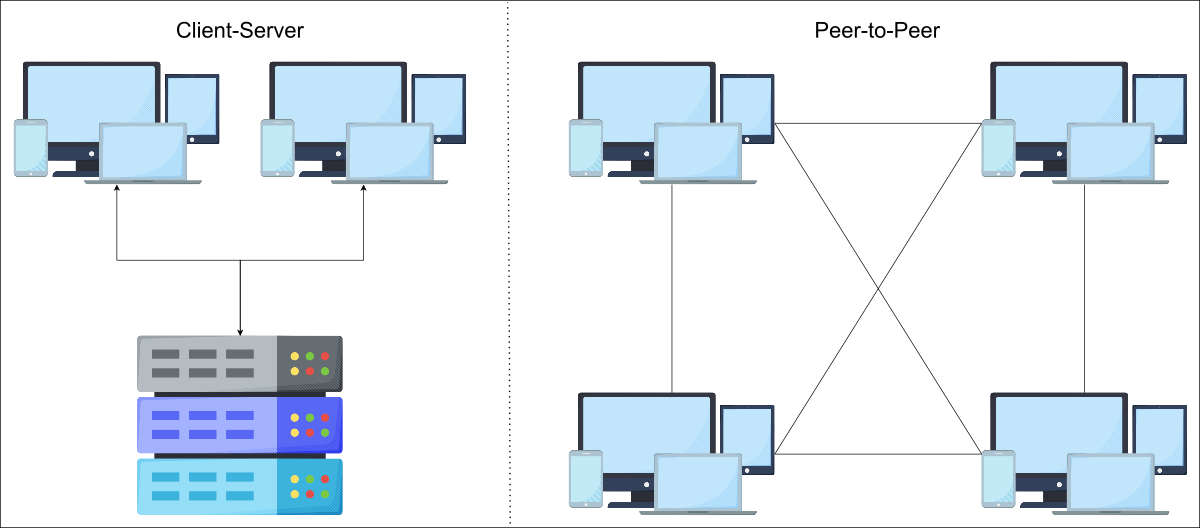
\includegraphics[width=0.5\textwidth]{Images/chapter_44/section_6123745074610176/5591275486707712.png}
 \caption{Client-server model vs. peer-to-peer model}
\end{figure}

The client-server model laid the foundation for the Internet and distributed systems, providing architectural styles such as MVC, microkernel, and numerous others. From this, we gained concepts such as load balancing (distributing incoming traffic), failover mechanisms (backups), and monitoring.
\\
Combining parallel computing concepts with computer networks provides the foundation for distributed systems.

\subsection{Distributed systems}\label{YrEBq65r3WOxRkOpUKzVJ}
\\
In today's interconnected world, the software we rely on is rarely confined to a single machine. Instead , it spans multiple computers, working together as a unified system. These are distributed systems.

\begin{figure}[htbp]
 \centering
 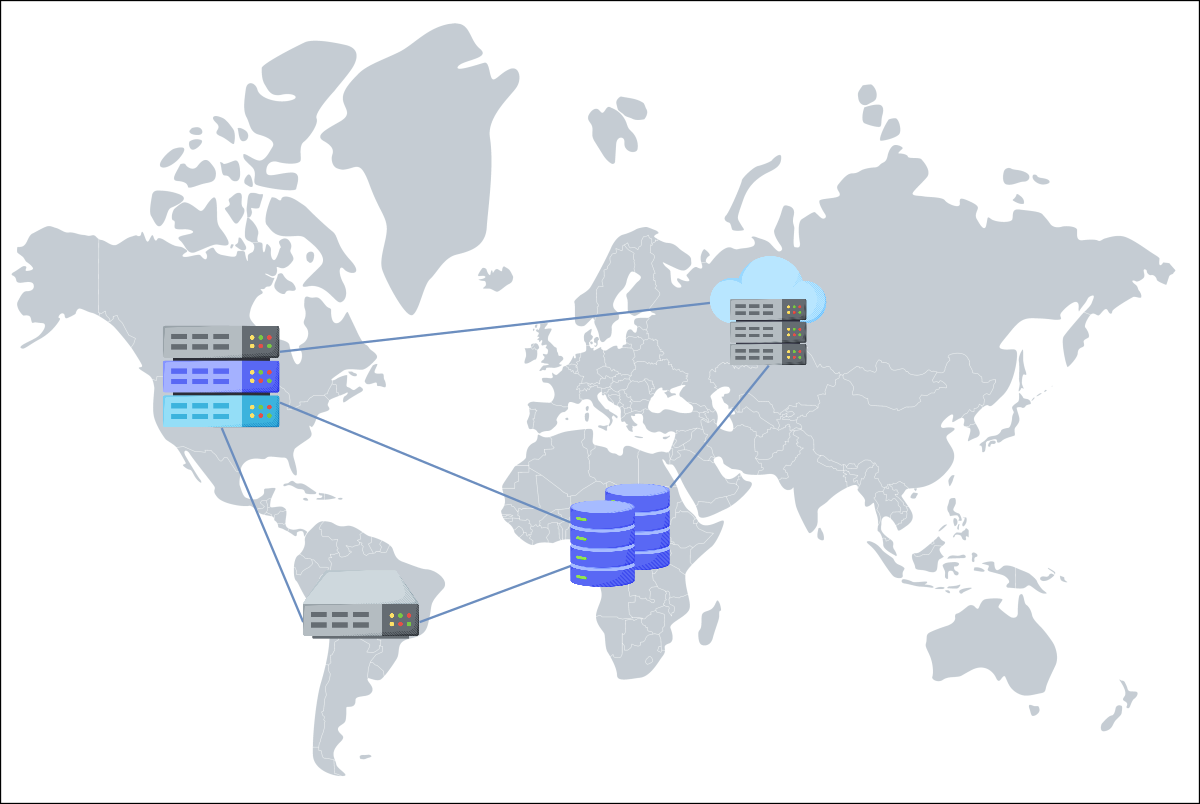
\includegraphics[width=0.5\textwidth]{Images/chapter_44/section_6123745074610176/6462332781592576.png}
 \caption{A distributed system}
\end{figure}

Distributed systems have several key characteristics that distinguish them from traditional, single-machine systems. These characteristics present challenges and opportunities for developers and users alike.

\subsubsection{Scalability}\label{Ma1EHaRAeix9_3wzzIkY-}
\\
One of the primary benefits of distributed systems is their ability to scale.
\\
Adding more computers to the system can increase its capacity to handle a greater number of users, data, or transactions. This scalability allows distributed systems to adapt to growing demands, ensuring a smooth user experience even as the workload increases.

\subsubsection{Availability}\label{Kpl9tt-wBZgAHi_ok7KHr}
\\
Distributed systems are designed to be highly available, meaning they should be accessible and operational even if some individual computers fail. This is achieved through redundancy and fault tolerance, where data and services are replicated across multiple machines.

\subsubsection{Replication and sharding}\label{Y7U-eLcK5ipiofvFxsMoI}
\\
To achieve scalability and availability, distributed systems often use \textbf{replication} (copying data across multiple machines) and \textbf{sharding} (dividing data into smaller pieces and distributing them across machines). These techniques help to distribute the load and ensure data remains accessible even in the face of failures.

\subsubsection{Consistency}\label{fO9OT1daV9Gd_hGAGdy2w}
\\
Distributed systems struggle to ensure data consistency across multiple machines.
\\
Strict consistency guarantees that every read sees the most recent write, even if it means sacrificing some availability. Eventual consistency prioritizes availability, allowing for temporary inconsistencies that are eventually resolved.

\subsubsection{Latency and performance}\label{X-dvHyZOJEVC2MbWf7pi_}
\\
In a distributed system, communication between computers takes time, introducing latency. This can impact the system's overall performance. Therefore, careful design and optimization are necessary to minimize latency and ensure a responsive user experience.

\subsubsection{Concurrency and coordination}\label{xorjCJYBRoMcxWCnKnOpI}
\\
Distributed systems often involve multiple processes or threads running concurrently across different machines. This can lead to complex interactions and race conditions, where the outcome of an operation depends on the timing of events.
\\
Coordination mechanisms are necessary to ensure that the system operates correctly in concurrent situations.
\begin{quote}
\textbf{Note:} Race conditions are a common problem when creating parallel applications. Knowing their mitigation strategies, such as locks, mutex, semaphores, etc., is imperative.
\end{quote}
\subsubsection{Security and privacy}\label{Ucdr3m_gbB1g7sF1PId_z}
\\
Due to their larger attack surface, distributed systems can be more vulnerable to security threats than single-machine systems. Implementing robust security measures, such as authentication(The process of verifying the identity of a user, device, or system attempting to access a network or resource, ensuring they are who they claim to be.), authorization(The process of determining and granting appropriate permissions and access levels to authenticated users, devices, or systems based on their roles and privileges.), and encryption(The process of converting plain text or data into a scrambled, unreadable format (ciphertext) using a cryptographic algorithm and key to protect its confidentiality.), is crucial to protect the system and its data from unauthorized access.

\subsubsection{Monitoring and observability}\label{DT7U704_Np7lPBvtwf_3t}
\\
Monitoring the health and performance of a distributed system is crucial for identifying and addressing issues before they impact users. Observability tools provide operators with insights into the system's behavior, helping them understand what's happening and why.

\begin{figure}[htbp]
 \centering
 
\includegraphics[width=0.15\textwidth]{Images/chapter_44/section_6123745074610176/5195396999151616.png}
 
\end{figure}

\subsubsection{Resilience and error handling}\label{QuK6P3cBi3J0v9oH4Ev6d}
\\
Distributed systems are complex, and failures are inevitable. A resilient system is designed to withstand failures and recover gracefully, minimizing downtime and data loss. Effective error-handling mechanisms are essential for ensuring the system's reliability.

The 2010 Flash Crash, where the stock market plunged and rebounded rapidly due to algorithmic trading errors,~highlights distributed systems' potential risks and complexities.

Understanding the diverse challenges and opportunities of distributed systems sets the stage for the crucial next step: defining the system requirements. After all, a well-designed system begins with a clear vision of what it needs to achieve.

\subsection{Defining system requirements}\label{AGGqKq6eQ_SY3AgHMX2Jq}
\\
Just as an architect needs a detailed blueprint before constructing a building, software developers need a well-defined set of system requirements before building a software system. These requirements outline what the system should do (functional requirements) and how well it should do (non-functional requirements).

\subsubsection{Identifying functional requirements}\label{yD_irvDIwEeRmvgh-H_u2}
\\
Functional requirements describe the specific features and capabilities that the system must provide. They answer the question, ``What should the system do?'' Think of them as the user's wish list. For a social media app, functional requirements might include:

\begin{itemize}
\item
\protect\phantomsection\label{0ICczWeuO-yH539PPpQVK}
The ability to create a profile.
\item
\protect\phantomsection\label{U5Ux7YP0rzA1bDrOWt0cN}
The ability to post messages, photos, and videos.
\item
\protect\phantomsection\label{3jD0bfwOiaDLjYgTNgq5m}
The ability to follow other users.
\item
\protect\phantomsection\label{o1_pvYhD7yFYKo4vB-Wmj}
The ability to like and comment on posts.
\end{itemize}
\begin{quote}
\textbf{Educative byte:} Always prioritize user needs and business goals when defining system requirements.~A perfectly designed system that doesn't solve the right problem is ultimately useless.
\end{quote}
\\
Identifying these requirements involves close collaboration with stakeholders, including users, product managers, and business analysts. User stories, use cases, and other techniques can help capture and prioritize functional requirements.

\subsubsection{Identifying non-functional requirements}\label{UdPiDM4WcI6p90CEVFMEe}
\\
Non-functional requirements are often overlooked, but they are just as critical to the success of a system as functional requirements. These requirements define the qualities that make the system usable, reliable, and efficient. Examples of non-functional requirements include:

\begin{itemize}
\item
\protect\phantomsection\label{Beb0sXg99Muy9fCp32_um}
\textbf{Performance:} How fast the system should respond to requests.
\item
\protect\phantomsection\label{9DkMhvFu_m-KTq49taqd_}
\textbf{Scalability:} How well the system should handle increased workload.
\item
\protect\phantomsection\label{6iMRCwGVQksVIEusL01kf}
\textbf{Availability:} How often should the system be accessible?
\item
\protect\phantomsection\label{bvzF_Ynyz6GiBvU3bM7R2}
\textbf{Security:} How well the system should protect data and prevent unauthorized access.
\item
\protect\phantomsection\label{r51d-cq40MhaVlv9b9wLM}
\textbf{Usability:} How easy the system should be to use.
\end{itemize}
\\
Determining non-functional requirements requires a deep understanding of the system's context, its users, and the environment in which it will operate. It 's also important to be realistic and avoid setting unattainable goals.

\subsubsection{Scoping requirements}\label{5GFPf3L1agYT4xgriIS3w}
\\
Scoping is the process of defining the boundaries of our project. It involves deciding which requirements are in scope (i.e., will be addressed) and which are out of scope (i.e., will not be addressed). This is a crucial step, as it helps to manage expectations and prevent scope creep( The uncontrolled expansion of a project\textquotesingle s requirements or features beyond the original plan), where the project grows uncontrollably.
\begin{quote}
\textbf{Note:} This is essential for a successful System Design interview. If we can balance the scope of functional and non-functional requirements with the time constraints of the interview, we are on a path to success.
\end{quote}
\\
It's important to strike a balance when scoping functional and non-functional requirements. We don't want to overload the system with too many features, but we also don't want to sacrifice essential qualities like performance or security.

\subsubsection{Trade-offs}\label{R7ZcVpgBEkZT9ZSucPCFy}
\\
In an ideal world, we could have a feature-rich, highly performant, scalable, and secure system.
\\
But in reality, trade-offs are often necessary. For example, increasing the level of security might impact performance, or adding more features might make the system harder to use. The key is to prioritize the most important requirements and make informed decisions about acceptable trade-offs.
\\
This requires careful consideration of the system's goals, users, and the available resources.
\begin{quote}
\textbf{Note:} This is another key aspect that will distinguish a candidate in an interview. A seasoned engineer is expected to be able to weigh the trade-offs between different requirements, develop valid reasoning, and implement the right ones in the design.
\end{quote}

\begin{figure}[htbp]
 \centering
 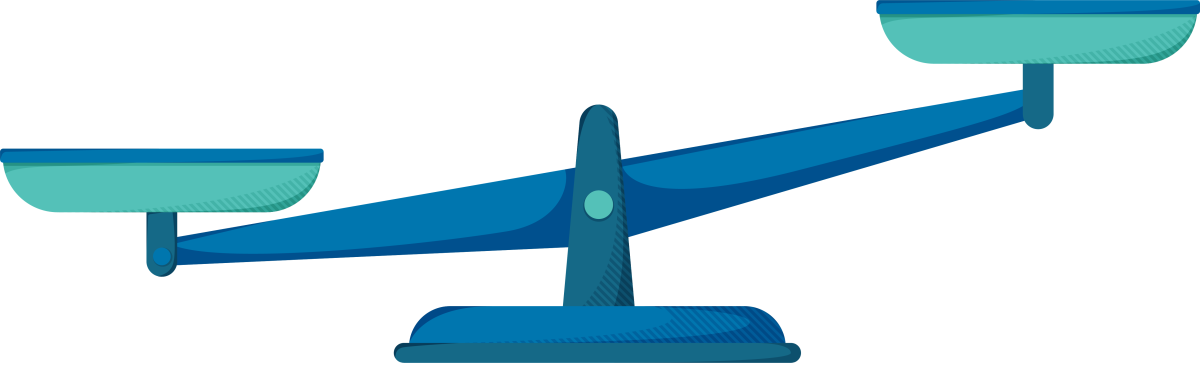
\includegraphics[width=0.15\textwidth]{Images/chapter_44/section_6123745074610176/4867731555483648.png}
 
\end{figure}

Defining system requirements is a complex but essential task. It requires clear communication, careful analysis, and the ability to make tough decisions. But when done well, it sets the stage for a successful project that delivers real value to its users.
\\
\textbf{Test your knowledge!}
\\
A development team is building a new mobile application that requires displaying complex, nested data from multiple sources on a single screen. They are highly concerned about minimizing data usage on slow mobile networks and want to avoid over-fetching. Which API architecture would be most suitable for these specific requirements?

\textbf{Question:}

Choosing API architecture

\textbf{Reference Answer:}

GraphQL allows clients to request exactly the data they need, which is ideal for minimizing data transfer on mobile networks and handling complex data queries.

\subsection{Conclusion}\label{hgHWeKpDUtIabBucygPdl}
\\
System Design is about understanding user needs, crafting a vision, and making informed decisions about bringing that vision to life. In this lesson, we\textquotesingle ve covered the foundational pillars that build upon our initial introduction: operating systems, computer networking, the specific challenges of distributed systems, and the process of defining requirements.
\\
In the next lesson, we will learn in detail about System Design trade-offs.

% End of section content